\documentclass{beamer}
\usepackage[utf8]{inputenc}

% Beamer Theme, might adapt
% https://hartwork.org/beamer-theme-matrix/
\usetheme{Madrid}
\usecolortheme{beaver}

%for colours e.g. \colorbox
\PassOptionsToPackage{usenames,dvipsnames}{xcolor}
\usepackage{xcolor}

%tables
\usepackage{longtable}
\usepackage{tabularx} 

\newcommand{\linebreakcellright}[2][c]{%
	\begin{tabular}[#1]{@{}r@{}}#2\end{tabular}}

\newcommand{\linebreakcellleft}[2][c]{%
	\begin{tabular}[#1]{@{}l@{}}#2\end{tabular}}

\newcommand{\linebreakcellcentre}[2][c]{%
	\begin{tabular}[#1]{@{}c@{}}#2\end{tabular}}


%Inline Code Snippets
\usepackage{listings}
\usepackage{color}

\definecolor{mygreen}{rgb}{0,0.6,0}
\definecolor{mygray}{rgb}{0.5,0.5,0.5}
\definecolor{mymauve}{rgb}{0.58,0,0.82}

\lstset{ 
	backgroundcolor=\color{white},   % choose the background color; you must add \usepackage{color} or \usepackage{xcolor}; should come as last argument
	basicstyle=\small,        % the size of the fonts that are used for the code
	breaklines=true,                 % sets automatic line breaking
	commentstyle=\color{mygreen},    % comment style
	extendedchars=true,              % lets you use non-ASCII characters; for 8-bits encodings only, does not work with UTF-8
	keepspaces=true,                 % keeps spaces in text, useful for keeping indentation of code (possibly needs columns=flexible)
	keywordstyle=\color{blue},       % keyword style
	language=Octave,                 % the language of the code
	morekeywords={parfor,pararrayfun, innerES},            % if you want to add more keywords to the set
	numbersep=5pt,                   % how far the line-numbers are from the code
	numberstyle=\tiny\color{mygray}, % the style that is used for the line-numbers
	rulecolor=\color{black},         % if not set, the frame-color may be changed on line-breaks within not-black text (e.g. comments (green here))
	showspaces=false,                % show spaces everywhere adding particular underscores; it overrides 'showstringspaces'
	showstringspaces=false,          % underline spaces within strings only
	showtabs=false,                  % show tabs within strings adding particular underscores
	stepnumber=1,                    % the step between two line-numbers. If it's 1, each line will be numbered
	stringstyle=\color{mymauve},     % string literal style
	tabsize=2,	                   	 % sets default tabsize to 2 spaces
}





% for pseudocode
\usepackage{amsmath}
\usepackage{algorithm}
\usepackage[noend]{algpseudocode}
\makeatletter
\def\BState{\State\hskip-\ALG@thistlm}
\makeatother

\title[jeff\textunderscore junior]{3 Axis Robot following a Laserpointer by using Stereovision and Templatematching}

\author[jwu, nsc]{Johannes Wüstner, Nicolai Schwartze}

\date{\today}

\begin{document}
\maketitle

\section{Introduction}
\frame{\tableofcontents}

\begin{frame}{Project Description}

\begin{itemize}
	\item construct a 3-axis robot with camera/laser tool
	\item calculate the backwards kinematic 
	\item program robot functions in C-DLL
	\item calibrate 3D camera system
	\begin{itemize}
		\item camera projection matrix
		\item hand-eye calibration
	\end{itemize}
	\item detect laser point on white flip-chart
	\item computer vision using OpenCV and Python
	\item drive with red robot laser to green user laser
\end{itemize}

\end{frame}


\section{Design}
\frame{\tableofcontents[currentsection]}

\begin{frame}{Task}
\begin{itemize}
	\item design a 3-axis robot in SolidWorks \\
	\item assemble the parts \\
	\item using Dynamixel MX-64AT motors \\
	\item attach camera/laser tool \\
\end{itemize}


\end{frame}


\begin{frame}{Result}

\begin{center}
	\begin{tabular}{ c c }
		  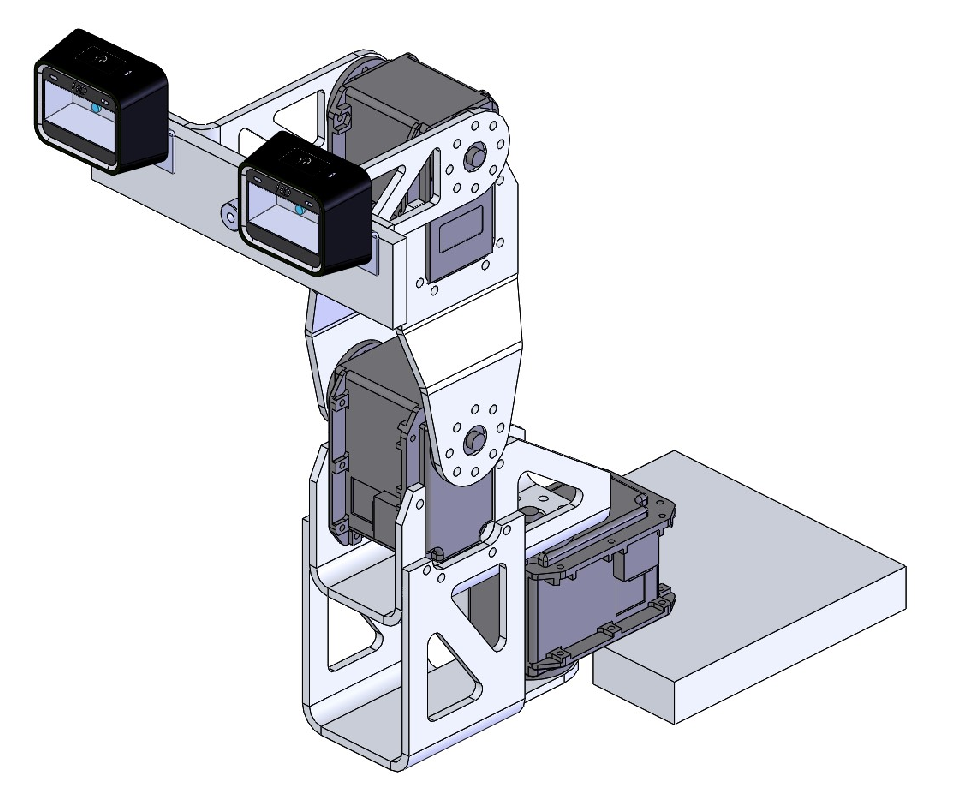
\includegraphics[width=\textwidth,height=0.45\textheight,keepaspectratio]{images/robot_3d_front.pdf} & 
		  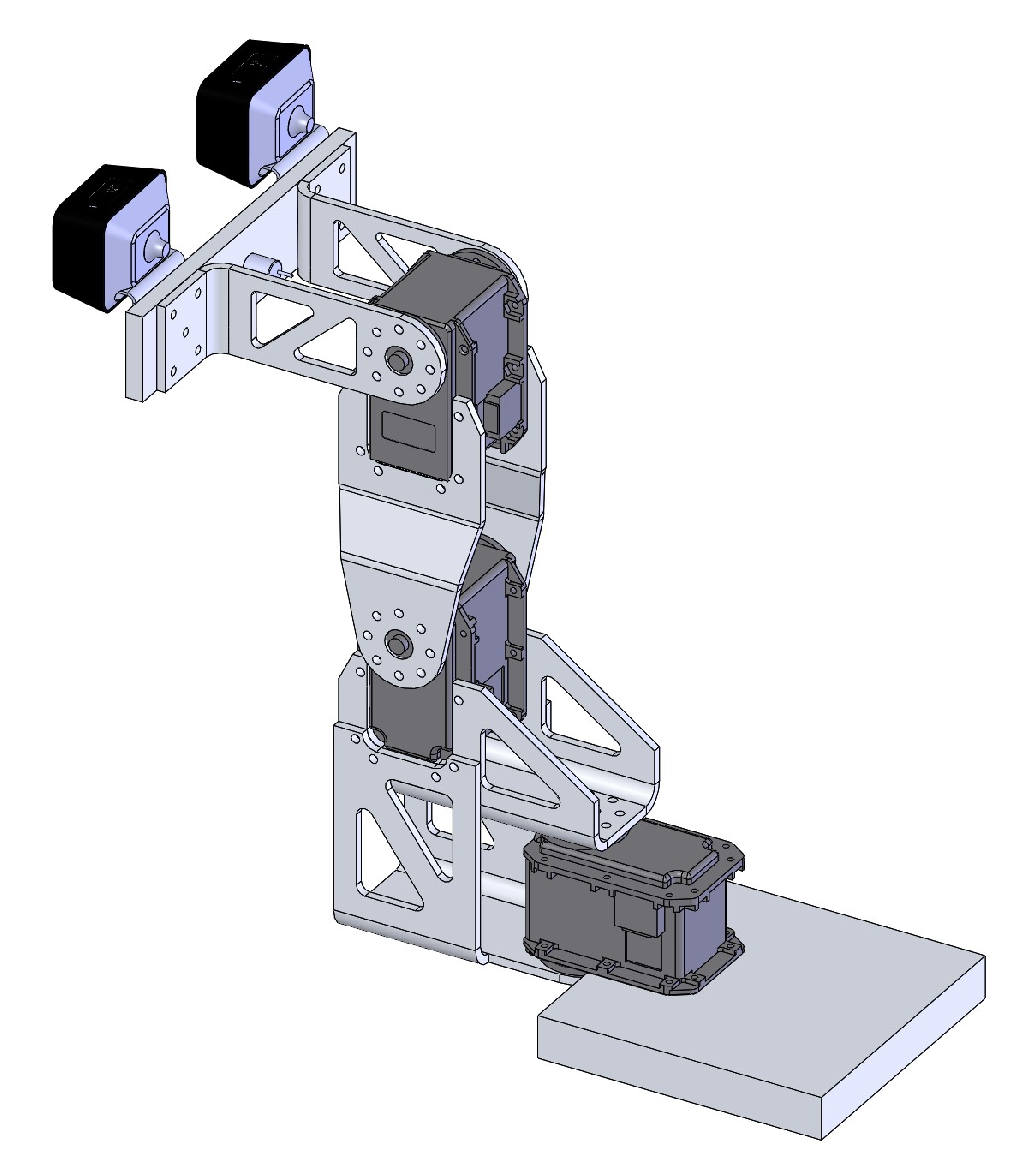
\includegraphics[width=\textwidth,height=0.5\textheight,keepaspectratio]{images/robot_3d_side.pdf} 
	\end{tabular}
\end{center}



\end{frame}



\section{Calculation}
\frame{\tableofcontents[currentsection]}

\begin{frame}{Task}

\begin{itemize}
	\item generate robot-backwards kinematic \\
	\item develop equation for setting angle of motor \\
	\item establish transformation matrix for hand-eye coordination \\
\end{itemize}

\end{frame}

\begin{frame}{Problem}

\begin{itemize}
	\item backwards kinematic
	\begin{itemize}
		\item establish DH parameter $\rightarrow$ transformation matrix TCP to robot base
	\end{itemize}
	\item setting motor angle
	\begin{itemize}
		\item only need two DOF $\rightarrow$ overdetermined
	\end{itemize}
	\item hand-eye coordination
	\begin{itemize}
		\item estimate the right distance camera to TCP
	\end{itemize}
\end{itemize}

\end{frame}

\begin{frame}{Solution I}

\begin{columns}[T] % align columns
	\begin{column}{.48\textwidth}
		\begin{center}
			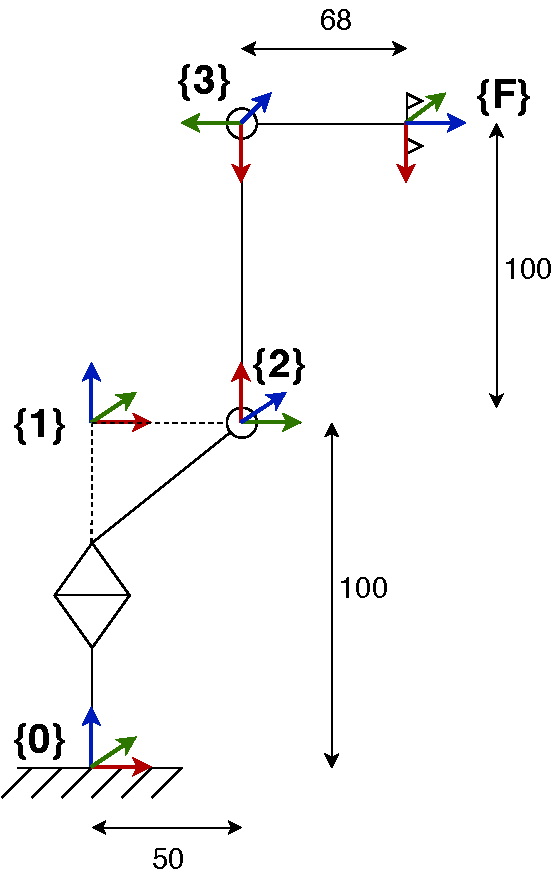
\includegraphics[width=\textwidth,height=0.8\textheight,keepaspectratio]{images/robot_axis_coord.pdf}
		\end{center}
		
	\end{column}%
	\hfill%
	\begin{column}{.45\textwidth}
		~\\~\\~\\
		\begin{center}
			\begin{tabular}{ c c c c c }
				$i$ & $\alpha_{i-1}$ & $a_{i-1}$ & $d_i$ & $\theta_{i-1}$\\ 
				\hline
				1 & 0 & 0 & 100 & $\theta_0$\\  
				2 & -90 & 50 & 0 & $\theta_1 - 90$\\ 
				3 & 0 & 100 & 0 & $\theta_2 + 180$\\ 
				F & 90 & 0 & 68 & $0$
			\end{tabular}
		\end{center}

	\end{column}%
\end{columns}


\end{frame}

\begin{frame}{Solution II}

\begin{equation}
\theta_0 = arctan(\frac{Y_0}{X_0})
\end{equation}

\begin{equation}
\theta_1 = 0.0
\end{equation}

\begin{equation}
\theta_2 = -1 \cdot arctan \left( \frac{ Z_0 - 100 - 100 cos(\theta_1)}{\sqrt{X_{0}^{2} + Y_{0}^{2}} - 50 - 100 sin(\theta_1)} \right)
\end{equation}

\end{frame}



\section{Camera Calibration}
\frame{\tableofcontents[currentsection]}

\begin{frame}{Task}

\begin{itemize}
	\item calculate camera matrix for both single cameras \\
	\item estimate translation and rotation between cameras \\
\end{itemize}


\end{frame}

\begin{frame}{Problem}

\begin{itemize}
	\item unstable against repetition \\
	\item chessboard must not have the same hight and width \\
	\item three quality control measures: 
	\begin{itemize}
		\item plausibility: translation vector between cameras
		\item measure actual 3D points 
		\item comparison with matlab
	\end{itemize}
\end{itemize}


\end{frame}

\begin{frame}{Solution}
\begin{center}
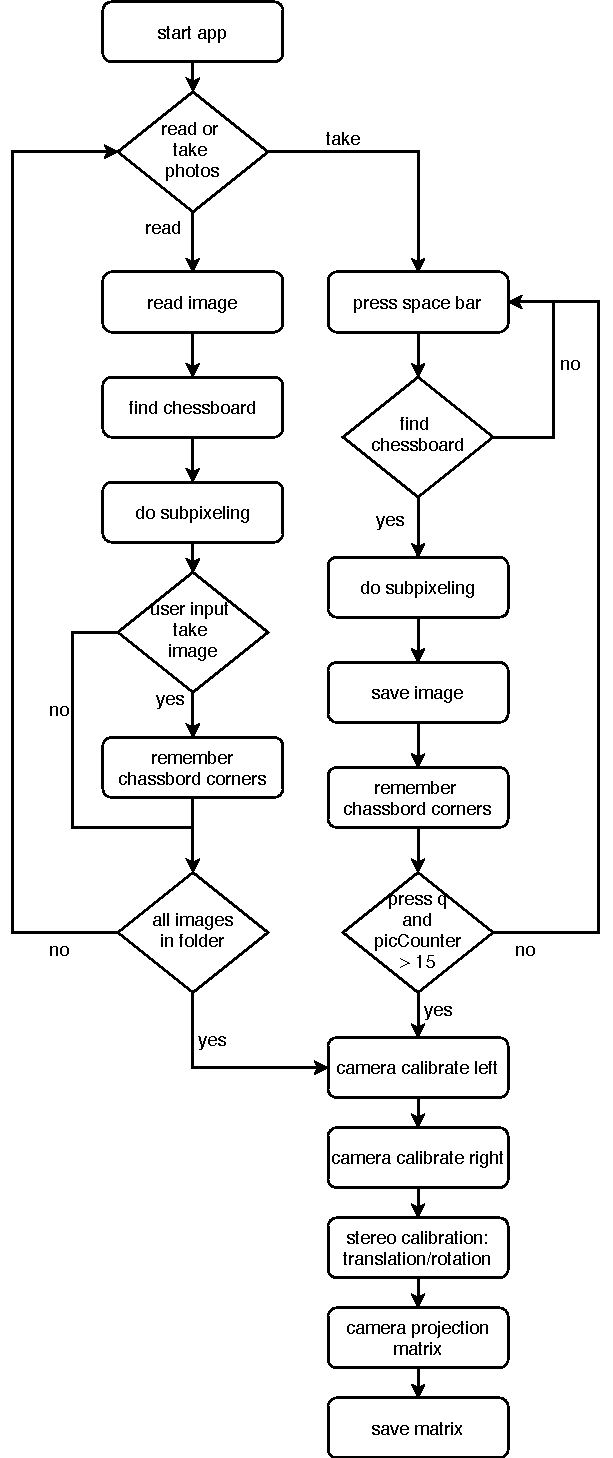
\includegraphics[width=\textwidth,height=0.85\textheight,keepaspectratio]{images/camera_calibration_app_flowchart.pdf}
\end{center}
\end{frame}



\section{Laser Point Detection}
\frame{\tableofcontents[currentsection]}

\begin{frame}{Task}

\begin{itemize}
	\item detect green laser point
	\item detect red laser point (not used; would be helpful for controller)
\end{itemize}


\end{frame}

\begin{frame}{Problem}

\begin{itemize}
	\item first idea: use threshold for colour of laser
	\item detect contour 
	\item calculate centre of mass 
	\item problem: unstable against other lighting conditions
	\bigskip
	\item red laser point too small
	\item use laser with adjustable focal length 
\end{itemize}


\end{frame}

\begin{frame}{Solution}

\begin{itemize}
	\item use template matching
	\item created template calibration app before every run
	\item more stable against lighting conditions
	\item but can only work on specified background (like a flip-chart)
\end{itemize}
~\\
using the CV\textunderscore TM\textunderscore CCOEFF\textunderscore NORMED

\begin{equation}
R(x,y) = \frac{\sum_{x',y'} (T'(x',y') \cdot I'(x + x', y + y'))}{\sqrt{\sum_{x',y'} T'(x',y')^{2} \cdot \sum_{x',y'} I'(x + x', y + y')^{2}}}
\end{equation}
~\\
also works for coloured images, this equation is applied for every channel


\end{frame}



\section{Conclusion, Further Work}
\frame{\tableofcontents[currentsection]}

\begin{frame}{Summary, Further Work}

\begin{itemize}
	\item works (sort of) but slow convergence
	\item overshooting 
	\item resting offset 
	\item not using $\theta_1$
	\item 3 USB ports needed - opencv does not find camera on hub
	\item red laser uses loads of batteries $\frac{220 mAh}{45 mA} = 4.8 h$
	\bigskip
	\item implement controller 
	\item correct laser offset to align with axis $\theta_2$
	\item use undistort before calculateing 3D point
	\item power supply for laser
\end{itemize}

\end{frame}



\end{document}